\documentclass[11pt]{article}
\usepackage[onehalfspacing]{setspace}
\usepackage{natbib} 
\usepackage{ocencfd}
\usepackage{graphicx}
\usepackage{parskip}
\begin{document}
\begin{titlepage}
\title{Gompertz Model Out-Performs Phenomenological and Other Mechanistic Models in Fitting Bacterial Population Growth Data}
\author{Jooyoung Ser}
\newcommand{\HRule}{\rule{\linewidth}{0.5mm}} % Defines a new command for the horizontal lines, change thickness here

%----------------------------------------------------------------------------------------
%	LOGO SECTION
%----------------------------------------------------------------------------------------


\includegraphics[width=8cm]{images/logo.eps}\\[1cm] 
 
%----------------------------------------------------------------------------------------

\center % Center everything on the page

%----------------------------------------------------------------------------------------
%	HEADING SECTIONS
%----------------------------------------------------------------------------------------

\textsc{\LARGE MSci CMEE Mini-Project}\\[1.5cm] % Name of your university/college
\textsc{\Large Imperial College London}\\[0.5cm] % Major heading such as course name
\textsc{\large Department of Life Sciences, Silwood Park}\\[0.5cm] % Minor heading such as course title

%----------------------------------------------------------------------------------------
%	TITLE SECTION
%----------------------------------------------------------------------------------------
\makeatletter
\HRule \\[0.6cm]
{ \huge \bfseries \@title}\\[0.6cm] % Title of your document
\HRule \\[1.5cm]
 
%----------------------------------------------------------------------------------------
%	AUTHOR SECTION
%----------------------------------------------------------------------------------------
\Large\@author\\[3cm] % Your name

%----------------------------------------------------------------------------------------
%	DATE SECTION
%----------------------------------------------------------------------------------------

{\large \today}\\[2cm] % Date, change the \today to a set date if you want to be precise

\vfill % Fill the rest of the page with whitespace

\end{titlepage}

	%New section is created
    \section{Abstract}
	\textbf{Model selection in ecology is a powerful alternative to hypothesis testing. In this study I fit bacterial population growth data using a large data from multiple literature sources using different mathematical model. After splitting the data into unique combinations of citation, medium, temperature and species, they were fit with all models. The mechanistic models tested required random sampling of parameters for optimal fits. The fit of each of the models were compared using Akaike's Information Criterion and the Bayesian Information Criterion as model selection methods. I found that Gompertz model out-performed the other models in ability to fit the bacterial population growth data. This indicates the importance of considering biological parameters in modelling population growth data. This study also highlights future directions to expand the scope of this study including other relevant mechanistic models and alternatives to method selection approaches.}
	
	\section{Introduction}
	%Plain text is just written directly in this document like this:
	Population biology as a field of research is not new. However multiple approaches to understanding population growth have been constantly developing. Population biology can be divided into two main areas of research: population genetics and population ecology. Population genetics refers to the study of genotypes and phenotype and how they reflect life histories and population density. In contrast, population ecology describes how and why factors affect populations. An important distinction between population genetics and population ecology is that population genetics considers evolution as a constant factor whereas population ecology ignores the effects of evolution. \citep{levins1966strategy}. Studying population ecology allows us to understand how organisms within ecosystems interact with each other as well as their environment. It also gives us insight into how these populations may change from the influence of external drivers like climate change and other environmental factors \citep{snider2013}. Previously, the main approach to studying population ecology was through hypothesis testing. A null hypothesis had to be statistically rejected to inform new scientific ideas. A more recent approach adopted in the fields of evolution and ecology is model selection. This method allows us to draw inferences from either one hypothesis or from multiple competing hypotheses. Model selection has clear advantages over hypothesis testing such as being able to consider more than one hypothesis and the ability to rank and weight models \citep{johnson2004model}. Mathematical models can be divided into two groups: mechanistic and phenomenological. Phenomenological models use mathematical functions that fit the data to make biological inferences. On the other hand, mechanistic models have underlying biological theories: components of the model describe specific biological processes. Therefore, often the parameters of mechanistic models describe underlying biological mechanisms without specifically referencing data \citep{white2019should}.
	
	The principal aim of this study is to find the mathematical model that best fits the bacterial population growth data. In addition, comparing the fit of different types of mathematical models, phenomenological and mechanistic, was an underlying aim in this study. In other words, comparing the functionality of using biologically derived parameters in modelling. Three polynomial linear models were modelled as the phenomenological models and the logistic growth model \citep{verhulst1838notice} and Gompertz model \citep{zwietering1990modeling} were the mechanistic models. 
	
    \section{Methods}
    \subsection{Data Preparation}
    The data I used in this study was a culmination of data from  different literature and therefore  were produced under different experimental designs. For example, there were a total of 45 different bacterial species, 18 different mediums and 4 different approaches to measuring population growth in the data.  The data had a total of 4397 observations. Using R, negative values of time and measures of population growth were removed to prevent potential errors in model fitting leaving the data with 4273 observations. In order to understand the effects of potential factors, the data was then divided into specific combinations of medium, temperature, species and citation. Ultimately, there were 285 unique combinations of these factors and these 285 smaller data sets were then individually fit with the mathematical models.
    
    \subsection{Models}
    A combination of 5 mathematical models were used to fit the data. 3 polynomial models: linear, quadratic and cubic, were used as well as the Logistic Growth model and Gompertz model. The linear, quadratic and cubic models are phenomenological models whereas the logistic growth and Gompertz model are mechanistic models. 
    
    \subsubsection{Logistic Model}
    The logistic growth model was developed as a generalisation of the exponential growth model with consideration of maximum capacity of populations in a series of papers published by Verhulst in 1838 \citep{bacaer2011verhulst}. The equation I used for the logistic growth model is shown below:
    
    \[ \scalebox{2}{$\displaystyleN_t = \frac{N_0Ke^{rt}}{K + N_0(e^{rt}-1)}$} \]
    where:
    \begin{description}
    \item[$N_{t}$] is population size at time $t$
    \item[$N_{0}$] is initial population size
    \item[$r$] is maximum growth rate
    \item[$K$] is carrying capacity
    \end{description}
    
    \subsubsection{Gompertz Model}
    The Gompertz model was developed by Benjamin Gompertz in his 1825 paper. The Gompertz model is a sigmoidal function that describes population growth rate to be slowest in the beginning and at the end \citep{gompertz1825xxiv}. The parameters of the Gompertz model mainly differs from the logistic model in the consideration of the lag phase of bacterial growth. The equation I used for the Gompertz model is shown below:
   
    \[ \scalebox{2}{$\displaystyle log(N_t)= N_0 + (N_{max} - N_0)e^{-e^{r_{max}exp(1)\frac {t_{lag}-t}{(N_{max}-N_0)log(10)}+1}}$} \]
    where:
    \begin{description}
    \item[$N_{t}$] is population size at time $t$
    \item[$N_{0}$] is initial population size
    \item[$r_{max}$] is maximum growth rate
    \item[$K$] is carrying capacity
    \item[$t_{lag}$] is the lag phase
    \end{description}
    
    \subsection{Model Fitting}
    All the models were fit in R. The mechanistic models require adequate starting values for  all the parameters. In order to find the optimal starting values for these two models, I conducted random sampling around estimates of the starting values to see which starting values allowed the models to successfully fit the most data. The random parameters were simulated 100 times for each of the 285 unique data sets for both models and then the optimal starting values were used to fit the data.
    
    \subsubsection{Logistic Model}
    The logistic model had 3 parameters that were selected through random sampling: carrying capacity $K$, growth rate $r$ and initial population size $N_0$. The random values from which the parameters were selected were normally distributed around a mean value for carrying capacity and initial population size. The mean values for carrying capacity and initial population size were the maximum and minimum population values for each 285 data sets respectively. The randomly generated starting values for growth rate were uniformly distributed between the bounds $10^{-10}$ and $10^{-2}$.
    
    \subsubsection{Gompertz Model}
    The Gompertz model had 4 parameters that were selected through random sampling: carrying capacity $K$, growth rate $r$, initial population size $N_0$ and lag phase $t_{lag}$. Like the logistic model, the random values from which the growth rates were selected had a uniform distribution bound between $10^{-10}$ and $10^{-2}$. In addition, the random values for carrying capacity $K$ and initial population size $N_0$ were normally distributed around the maximum and minimum population values for each 285 data respectively. The lag phase parameter $t_{lag}$ random values were also normally distributed around a calculated mean value.
    
    
    \subsection{Model Selection}
    Model selection was carried out using the Akaike Information Criterion (AIC) \citep{akaike1977entropy} and the Bayesian Information Criterion (BIC) \citep{schwarz1978estimating}. I used both AIC and BIC to determine which of the 100 random parameters best fit each of the 285 data sets for both models. I then used AIC and BIC to compare the all the models, including the phenomenological models, to find which of them best fit the data. Both AIC and BIC penalise parameters to compensate for over-fitting but BIC penalises model complexity more heavily. There is much confusion in the literature as to which of these model selection approaches are better despite them often yielding the similar results \citep{aho2014model}. In light of this, I decided to use both model selection criteria in this study.
    
    \subsubsection{Akaike Information Criterion (AIC)}
    The lower the AIC value, the better the model fits the data. As minute differences between AIC values cannot confidently infer which is the better model a cut off point of two AIC values was adopted. Therefore, a model was only deemed the better fit if was more than two AIC values lower than the next model.
    \[AIC = n + 2 + nlog(\frac{2 \pi }{n}) +nlog(RSS) + 2p\]
    where:
    \begin{description}
    \item[$n$] is sample size
    \item[$p$] is number of parameters
    \item[$RSS$] is residual sum of squares
    \end{description}
    
    \subsubsection{Bayesian Information Criterion (BIC)}
    Like AIC, the lowest BIC value indicates the best fit model. I also adopted the two BIC value cut off point for this model selection approach. 
      \[BIC = n + 2 + nlog(\frac{2 \pi }{n}) +nlog(RSS) + plog(n)\]
    where:
    \begin{description}
    \item[$n$] is sample size
    \item[$p$] is number of parameters
    \item[$RSS$] is residual sum of squares
    \end{description}
    
    \subsection{Computing Tools}
    R version 4.2.2 was used to conduct the data preparation, model fitting, model selection and plotting. I used R more than python as I have more experience using R. Bash shell scripting is used to compile the text scripts using Latex.
    
    \section{Results}	
    \subsection{Model Selection}
        \begin{figure}[h!]
	        \centering
  	    	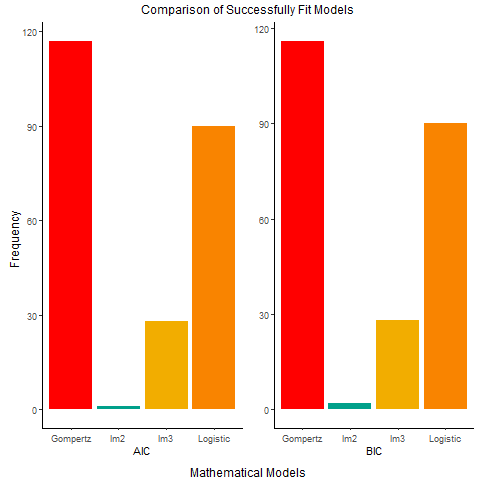
\includegraphics[scale = 0.5]{images/fig_1.png}
  		    \caption{Abbreviations: lm2 = quadratic linear model, lm3 = cubic linear model. Bar plot showing the best models for the 285 unique data sets from bacterial population growth data according to AIC and BIC model selection methods. Linear model did not fit any of the data sets the best. Data analysis and plotting carried out in R}
  		    \label{Figure 1}
    	\end{figure}
    
    The Gompertz model was found to fit the most data sets according to both AIC and BIC model selection approaches (Fig. 1). Under AIC, the Gompertz model fits 117 of 285 data sets the best amongst the other models. Under BIC, the Gompertz model fits 116 of 285 data sets the best. In both model selection approaches the model that next best fits the data is the logistic growth model with 90 of the 285 data sets being best fit by the logistic growth model. The linear model did not fit any of the data sets the best. This shows that the mechanistic models outperformed all the phenomenological models under both AIC and BIC model selection methods. 49 of 285 data sets under both model selection methods were not assigned a best fitting model due to the predetermined cut-off point of two AIC/BIC values.
    
	
    \section{Discussion}
    The results indicate a clear advantage of considering biological factors in mechanistic models, of which the Gompertz model best fit the largest proportion of the bacterial growth data. There are a multitude of reasons why the Gompertz model was not able to fit more of the data sets. One of these reasons could be that the starting values were unsuitable for the data. In particular, the lag phase $t_{lag}$ parameter is difficult to fit as they can vary between and even within species \citep{zwietering1992comparison}. A future direction that could solve this would be to test more randomly sampled parameters as 100 sets of random parameters may not have been sufficient to find the optimal starting values for the models. Another reason why models did not fit could be the discrepancies within the data itself. As the data come from different sources, they had differing experimental design and therefore inconsistency in the data is likely. A solution to overcome this would be to perform the same analyses at a bigger scale with more data.
    
   Although an aim of this study was to compare phenomenological and mechanistic models in modelling bacterial population growth data, an important detail to mention is that the logistic growth model and Gompertz model cannot be considered truly mechanistic. Despite accounting for some biological processes with parameters, the models are not completely derived from biological first principles. It is difficult to translate all physiological and environmental influences into an equation which makes true mechanistic models difficult to develop. Strictly speaking, this study compared the performance of phenomenological models and almost-mechanistic models. This complication could be alleviated by modelling multiple mechanistic in conjunction, however this is beyond the scope of this study. Examples of other mechanistic models to model population growth include a model suggested by Hutchinson in 1948. This mechanistic model implements the idea of developmental delays due to environmental feedback loops \citep{hutchinson1948circular}. An additional example of a mechanistic model to consider is Fisher's equation which accounts for diffusion of a spatially-extended unstructured population. Diffusion is unlikely to be an drawback in lab grown bacteria in petri dishes however it will better model bacterial colonies in the wild \citep{fisher1937wave}.
    
    On the other hand, the law of parsimony opposes complicated models that over-fit the data. The law of parsimony states that solving principles should not be complicated beyond necessity. In this case, a simpler model is preferred over models with numerous parameters \citep{re2002william}. This presents a dilemma in which population ecologists are forced to compromise between optimal fit of the data and excessive complexity. Finding this boundary where parsimony and fit are balanced also opens up another potential future direction.
    
     There is also room for improvement regarding model selection approaches. I chose an arbituary cut off point of at least a difference of 2 AIC/BIC values but bigger differences would indicate a stronger evidence to support a model's fit. By investigating the varying differences between AIC and BIC values, more insight into modelling bacterial population growth could be inferred. There is also a different type of AIC model selection which could improve the validity of this study. AICc is modified version of AIC which corrects for the effects of of small sample size. For that reason, AICc as may have been a more appropriate model selection approach in this study.
     
     In this study I demonstrated the ability of mechanistic models, in particular the Gompertz model, in fitting bacterial growth data. Results indicate that additional biological parameters allow the models to better model bacterial population growth behaviour. The powerful analytic tools that are AIC and BIC were also demonstrated as model selection approaches. However, despite the advantages of including biological parameters that make a model mechanistic, it is also important to consider the law of parsimony.
    
    \pagebreak
    \bibliographystyle{agsm}
	%Add bibliography at the end of document	
	\bibliography{miniproject_writeup}
	\label{bibsect}

\end{document} % This is the end of the document